\documentclass[11pt,a4paper]{article}

% -----------------------------
% PAQUETES
% -----------------------------
\usepackage[utf8]{inputenc}
\usepackage[T1]{fontenc}
\usepackage[spanish]{babel}
\usepackage{helvet}
\renewcommand{\familydefault}{\sfdefault}

\usepackage{geometry}
\usepackage{graphicx}
\usepackage{xcolor}
\usepackage{eso-pic}
\usepackage{enumitem}
\usepackage{parskip}
\usepackage{setspace}
\usepackage{ragged2e}

% Paquetes matemáticos
\usepackage{amsmath,amssymb,amsfonts,mathtools}

% -----------------------------
% MÁRGENES
% -----------------------------
\geometry{
    a4paper,
    left=2.3cm,
    right=2.3cm,
    top=6.0cm,
    bottom=3.0cm
}

\setstretch{1.08}
\setlength{\parindent}{0pt}

% -----------------------------
% RUTAS DE IMÁGENES
% -----------------------------
\newcommand{\HeaderImg}{imagenes/Header.jpg}
\newcommand{\FooterImg}{imagenes/footer.jpg}

% -----------------------------
% MEDIDAS DEL FORMATO
% -----------------------------
\newcommand{\BannerTopOffset}{4.5cm}
\newcommand{\FooterWidth}{\dimexpr\paperwidth-1.8cm\relax}

% -----------------------------
% HEADER Y FOOTER COMO FONDO
% -----------------------------
\AddToShipoutPictureBG{%
    % Header superior
    \AtPageUpperLeft{%
        \raisebox{-\BannerTopOffset}{%
            \includegraphics[width=\paperwidth]{\HeaderImg}%
        }%
    }%
    % Footer inferior
    \AtPageLowerLeft{%
        \hspace*{0.9cm}%
        \raisebox{0.55cm}{%
            \includegraphics[width=\FooterWidth]{\FooterImg}%
        }%
    }%
}

\pagestyle{empty}

% -----------------------------
% COMANDO PARA TÍTULO
% -----------------------------
\newcommand{\FormatoTitulo}[1]{%
    \begin{center}
        \vspace*{-0.4cm}
        {\fontsize{22}{24}\selectfont #1\par}
        \vspace{0.25cm}
        {\color[rgb]{0.35,0.23,0.95}\rule{8.2cm}{1.4pt}}
    \end{center}
    \vspace{1.2cm}
}

\begin{document}

\FormatoTitulo{Propuesta de proyecto de grado}

\begin{enumerate}[leftmargin=0.8cm,label=\arabic*.,itemsep=1.0em]

    \item \textbf{Título del Proyecto.}

    Segmentación automática de columna vertebral y vértebras en radiografías con escoliosis para entornos con recursos computacionales limitados.

    \item \textbf{Organización/Grupo de investigación.}

    El proyecto se enmarca en la \textbf{Maestría en Inteligencia Artificial (MAIA)} de la \textbf{Universidad de los Andes}, en el área de visión por computador aplicada a imágenes médicas.

    Este trabajo aborda un problema de salud digital: análisis automático de radiografías de columna para apoyar la evaluación de escoliosis. El grupo de trabajo está conformado por Jason Rosher Morrill, John Williams Morrill, David Alan Delgado Zarco y Octavio Esquivel Álvarez del Castillo, con acompañamiento académico de docentes e investigadores del programa MAIA en modelado de aprendizaje profundo, analítica de datos y evaluación experimental.

    \item \textbf{Contexto, problema y justificación. Impacto esperado.}

    \textbf{a) Situación actual y contexto.} La escoliosis es una deformidad tridimensional de la columna vertebral cuyo seguimiento clínico se realiza principalmente con radiografías anteroposteriores. En práctica médica, la severidad se cuantifica con el ángulo de Cobb, que requiere identificar manualmente vértebras límite y trazar líneas sobre placas terminales.

    \textbf{b) Problema a abordar.} El proceso manual introduce variabilidad interobservador y limita la reproducibilidad de las mediciones. Además, la segmentación automática en radiografías 2D es difícil por superposición de estructuras, variabilidad morfológica vertebral, diferencias de escala/campo de visión y ruido en anotaciones. Muchos enfoques actuales aprenden rasgos locales pero no incorporan explícitamente estructura topológica y geométrica de la columna.

    Formalmente, dada una radiografía \(I:\Omega\rightarrow\mathbb{R}\), con \(\Omega\subset\mathbb{R}^2\), se busca estimar:
    \[
    f_{\theta}: I \rightarrow Y,
    \]
    donde \(Y:\Omega\rightarrow\{0,1,\dots,C-1\}\) representa una máscara multiclase por vértebra. El problema de aprendizaje se plantea como:
    \[
    \theta^*=\arg\min_{\theta}\,\mathbb{E}_{(I,Y)\sim D}\left[\mathcal{L}(f_{\theta}(I),Y)\right].
    \]

    \textbf{c) Justificación e impacto esperado.} Se propone un modelo híbrido (CNN + TDA + Transformer multi-kernel) para mejorar la coherencia anatómica de la segmentación vértebra a vértebra y facilitar la estimación automática del ángulo de Cobb. Se espera reducir variabilidad de medición, aumentar reproducibilidad y habilitar herramientas de apoyo clínico y de tamizaje en contextos con recursos computacionales limitados.

    \item \textbf{Objetivos.}

    \textbf{Objetivo general.} Desarrollar un modelo híbrido basado en CNN, análisis topológico de datos y Transformers kernelizados para la segmentación automática de vértebras y la estimación del ángulo de Cobb en radiografías de columna vertebral.

\textbf{Objetivos específicos.}
\begin{itemize}[leftmargin=0.6cm]
    \item Implementar y comparar tres configuraciones experimentales: \textit{Baseline CNN}, \textit{CNN + Transformer} y \textit{CNN + TDA + Transformer multi-kernel}.
    \item Diseñar una estrategia de representación que combine rasgos convolucionales, descriptores topológicos y estructura geométrica para mejorar la segmentación vértebra a vértebra.
    \item Cuantificar el aporte de cada componente del modelo mediante estudios de ablación usando métricas de segmentación y error en la estimación del ángulo de Cobb.
    \item Evaluar la viabilidad computacional del enfoque propuesto en términos de tiempo de entrenamiento, tiempo de inferencia y consumo de recursos en entornos con capacidad limitada.
\end{itemize}

    \item \textbf{Estado del arte.}

    En segmentación médica, arquitecturas tipo U-Net y variantes como nnU-Net han establecido líneas base sólidas. Para columna y vértebras, trabajos recientes incorporan Transformers para capturar dependencias globales y mejorar consistencia anatómica, especialmente en CT con campo de visión variable.

    Se identifican dos líneas principales: (i) enfoques tipo DETR con \textit{query tokens} para etiquetado/segmentación vertebral, y (ii) integración de ViT/Swin en esquemas encoder-decoder tipo U-Net para segmentación densa. También existen propuestas con señales auxiliares (bordes, centroides) para reforzar separación entre vértebras.

    La limitación común es que la geometría y topología explícita suelen estar subrepresentadas: se usan centroides, bordes o codificación posicional, pero rara vez descriptores formales de homología persistente, números de Betti, curvatura o geodésicas dentro del embedding y de la atención. Esta brecha es más evidente en radiografías 2D, donde además se recurre con frecuencia a postprocesamientos heurísticos.

    El proyecto aborda ese vacío mediante tokens vertebrales enriquecidos con descriptores topológicos y geométricos, y atención multi-kernel informada por estructura anatómica.

    \item \textbf{Metodología y solución propuesta.}

    Se propone un pipeline con cinco etapas:
    \begin{itemize}[leftmargin=0.6cm]
        \item \textbf{Extracción local (CNN):} obtención de \textit{feature maps} y embeddings anatómicos a partir de la radiografía.
        \item \textbf{Enriquecimiento topológico (TDA):} construcción de complejos simpliciales (Vietoris-Rips) y extracción de descriptores topológicos vectorizados.
        \item \textbf{Componente geométrico (manifold):} incorporación de estructura geométrica intrínseca sobre el espacio de embeddings.
        \item \textbf{Transformer multi-kernel:} cada cabeza de atención opera con kernels distintos (p. ej., lineal, RBF, coseno/polinomial) según el espacio de representación (CNN, topológico, manifold).
        \item \textbf{Decodificación densa:} generación de máscara multiclase vértebra a vértebra y cálculo de métricas derivadas (como ángulo de Cobb).
    \end{itemize}

    Flujo funcional resumido del modelo:
    \[
    F = F_{\text{Dec}} \circ F_{\text{Trans}}^{\{k_h\}} \circ F_{\text{Top}} \circ F_{\text{CNN}}.
    \]

    Para una imagen de entrada \(I\in\mathbb{R}^{H\times W}\), el flujo de representación se describe como:
    \[
    I\xrightarrow{\phi}Z^{cnn}\xrightarrow{\tau}Z^{topo}\xrightarrow{k}\tilde{Z}\xrightarrow{\mathcal{T}}\hat{Y}.
    \]

    En la atención kernelizada por cabeza \(h\), se define:
    \[
    (K_h)_{ij}=k_h(t_i,t_j),\qquad
    A_h(i,j)=\frac{\exp((K_h)_{ij})}{\sum_{j'=1}^{n}\exp((K_h)_{ij'})},
    \]
    y
    \[
    \mathrm{head}_h(i)=\sum_{j=1}^{n}A_h(i,j)V_h(t_j).
    \]

    Como kernels candidatos se consideran, entre otros:
    \[
    k_{linear}(x_i,x_j)=x_i^\top x_j,\quad
    k_{RBF}(x_i,x_j)=\exp\left(-\frac{\|x_i-x_j\|^2}{2\sigma^2}\right),
    \]
    \[
    k_{poly}(x_i,x_j)=(x_i^\top x_j + c)^p.
    \]

    Para entrenamiento y experimentación, se utilizará una infraestructura escalable con planificador \textit{round robin}, ejecución paralela de \textit{workers}, \textit{early stopping} basado en eventos y trazabilidad en MLflow.

    \item \textbf{Exploración y descripción de los datos.}

    El dataset contiene radiografías anteroposteriores de columna de pacientes con y sin escoliosis, con diferentes niveles de anotación:
    \begin{itemize}[leftmargin=0.6cm]
        \item Radiografía original en escala de grises.
        \item Máscara binaria de columna.
        \item Segmentación multiclase por vértebra (etiquetas independientes).
        \item Curva espinal estimada a partir de la segmentación.
        \item Métricas clínicas asociadas (incluyendo ángulo de Cobb).
    \end{itemize}

    \textbf{Limitaciones y sesgos potenciales:} variabilidad en resolución/contraste, superposición de estructuras anatómicas en 2D, diferencias de morfología vertebral entre pacientes y posibles inconsistencias en anotaciones.

    \textbf{Estrategia de preparación:} estandarización de formato, control de calidad de etiquetas, partición entrenamiento-validación-prueba y definición de flujos de preprocesamiento orientados a mejorar robustez ante variaciones de escala y ruido.

    Además de las máscaras, el dataset incluye representaciones derivadas (curva espinal y overlays con métricas clínicas), lo cual permite evaluar consistencia anatómica global y no solo desempeño por píxel.

    \begin{center}
        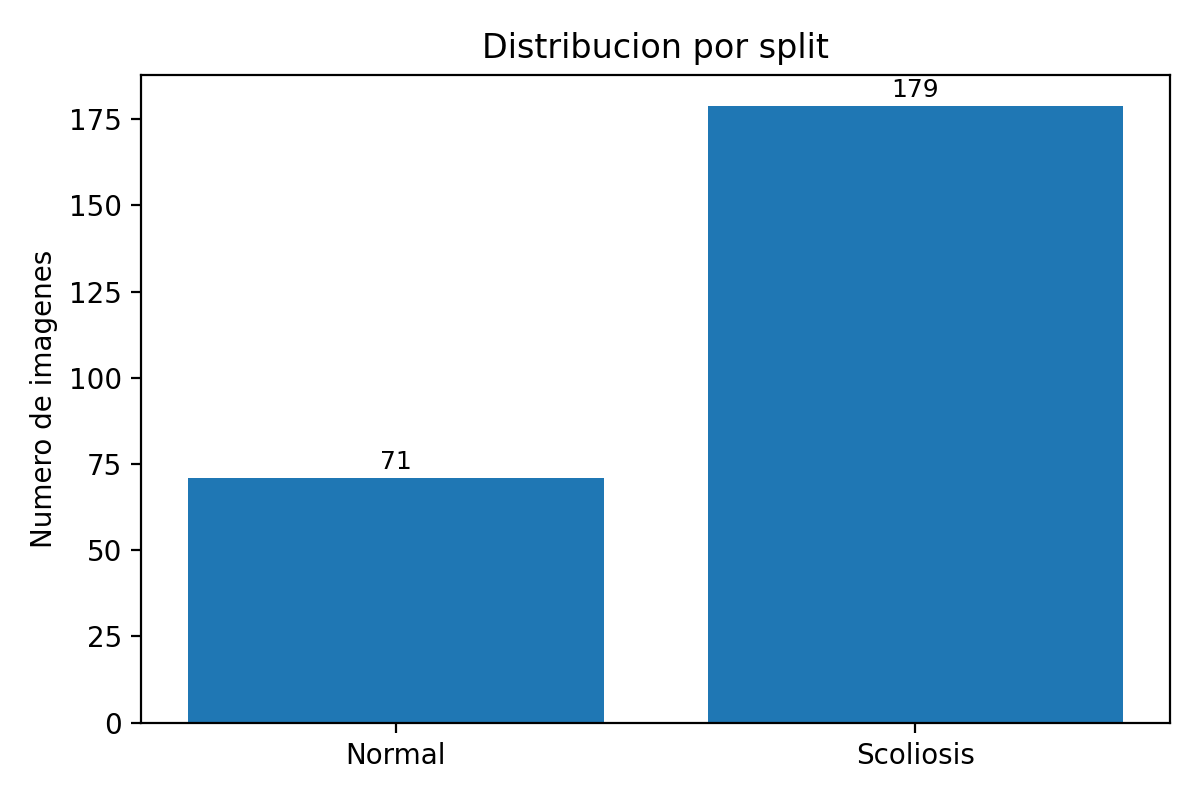
\includegraphics[width=0.48\linewidth]{analysis/figures/split_distribution.png}
        \hfill
        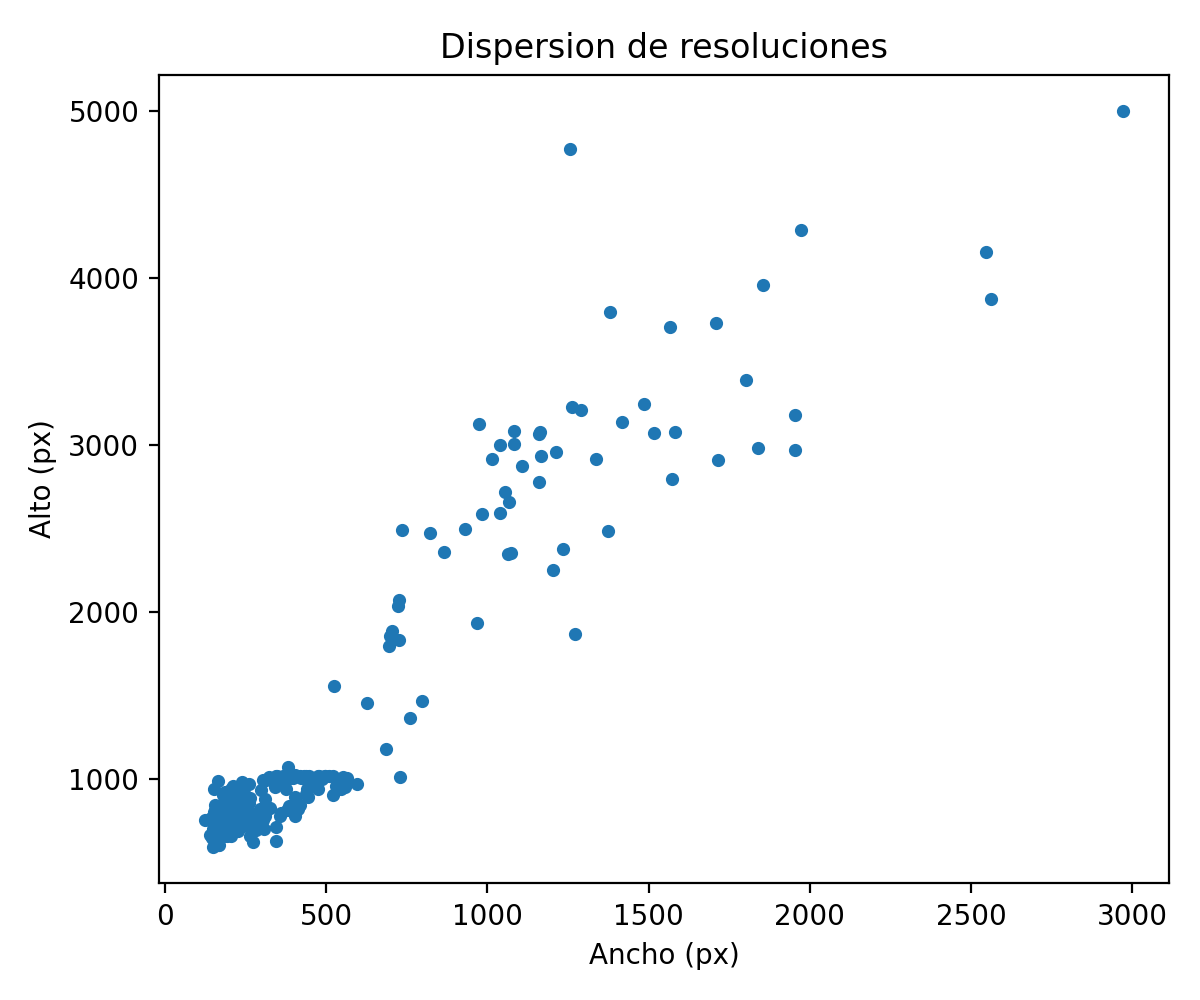
\includegraphics[width=0.48\linewidth]{analysis/figures/resolution_scatter.png}
    \end{center}
    \textit{Figura.} Diagnóstico exploratorio del dataset: distribución de muestras por clase y dispersión de resoluciones de las radiografías.

    \item \textbf{Consideraciones éticas.}

    El proyecto considera el uso responsable de datos médicos y la mitigación de riesgos de sesgo algorítmico:

    \begin{itemize}[leftmargin=0.6cm]

        \item \textbf{Privacidad.} El manejo de imágenes médicas (X-ray) conlleva una alta sensibilidad ética. Para garantizar la integridad de la información y cumplir con normativas de protección de datos:
        \begin{itemize}[leftmargin=0.6cm]
            \item \textbf{Anonimización:} se aplicarán protocolos estrictos para eliminar metadatos de identificación personal antes del entrenamiento.
            \item \textbf{Seguridad:} el procesamiento en la nube y el bus de mensajería (Pub/Sub, SQS) contarán con cifrado de extremo a extremo, evitando exposición o uso indebido de los datos.
        \end{itemize}

        \item \textbf{Sesgos.} Un desafío crítico en el desarrollo del modelo es el desequilibrio de clases en el dataset, donde la prevalencia de radiografías de columnas sanas sobre casos con escoliosis severa puede inducir un sesgo de normalidad.
        \begin{itemize}[leftmargin=0.6cm]
            \item \textbf{Sesgo identificado:} el modelo podría tender a clasificar erróneamente la mayoría de los casos como ``sin escoliosis''.
            \item \textbf{Mitigación:} se emplearán funciones de pérdida ponderadas (\textit{weighted loss functions}) para aumentar la importancia estadística de las clases minoritarias durante el entrenamiento.
        \end{itemize}

        \item \textbf{Impacto social.} Aunque la automatización de la segmentación vertebral y del cálculo del ángulo de Cobb puede mejorar la eficiencia clínica, existe preocupación legítima sobre el desplazamiento de tareas rutinarias realizadas por especialistas. El enfoque propuesto no busca sustituir al médico, sino funcionar como herramienta de soporte a la decisión clínica.

        \item \textbf{Transparencia y trazabilidad.} Dada la naturaleza de caja negra de muchas redes neuronales profundas, la arquitectura propuesta incorpora análisis topológico de datos y geometría diferencial para aportar interpretabilidad estructural.
        \begin{itemize}[leftmargin=0.6cm]
            \item El sistema permitirá visualizar la línea central estimada y los puntos anatómicos usados para el cálculo del ángulo de Cobb.
            \item Esta transparencia facilitará la auditoría del modelo y la comunicación comprensible de los resultados al personal médico y a los pacientes.
        \end{itemize}

    \end{itemize}

    \item \textbf{Evaluación y métricas.}

    La evaluación se realizará comparando tres configuraciones: \textbf{Baseline CNN}, \textbf{CNN + Transformer}, y \textbf{CNN + TDA + Transformer multi-kernel}.

    \textbf{Criterios y métricas principales:}
    \begin{itemize}[leftmargin=0.6cm]
        \item Calidad de segmentación por vértebra (p. ej., Dice y métricas complementarias de precisión/F1 según la configuración experimental).
        \item Coherencia anatómica global de la segmentación.
        \item Error en la estimación del ángulo de Cobb respecto a la referencia disponible.
        \item Eficiencia computacional y estabilidad de entrenamiento.
    \end{itemize}

    Se incluirán estudios de ablación para cuantificar el aporte de descriptores topológicos, kernels de atención y componente geométrico. El diseño experimental contempla tres escenarios: \textbf{Baseline CNN}, \textbf{CNN + Transformer} y \textbf{CNN + TDA + Transformer multi-kernel}, con validación comparativa bajo el mismo protocolo de partición de datos.

    Como referencia del mecanismo base de atención contextual, también se considerará la formulación estándar:
    \[
    \mathrm{Attention}(Q,K,V)=\mathrm{softmax}\left(\frac{QK^\top}{\sqrt{d_k}}\right)V.
    \]

    \begin{center}
        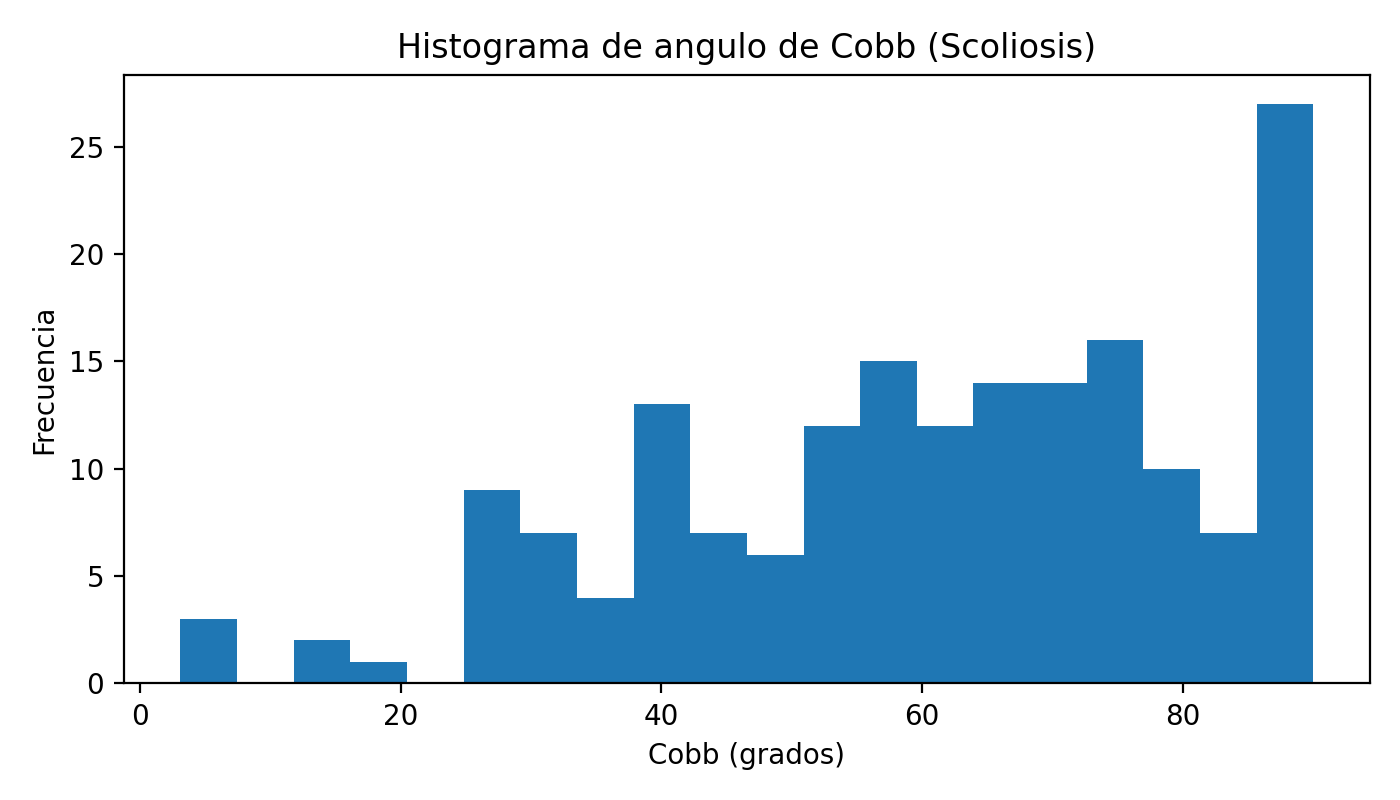
\includegraphics[width=0.48\linewidth]{analysis/figures/cobb_histogram.png}
        \hfill
        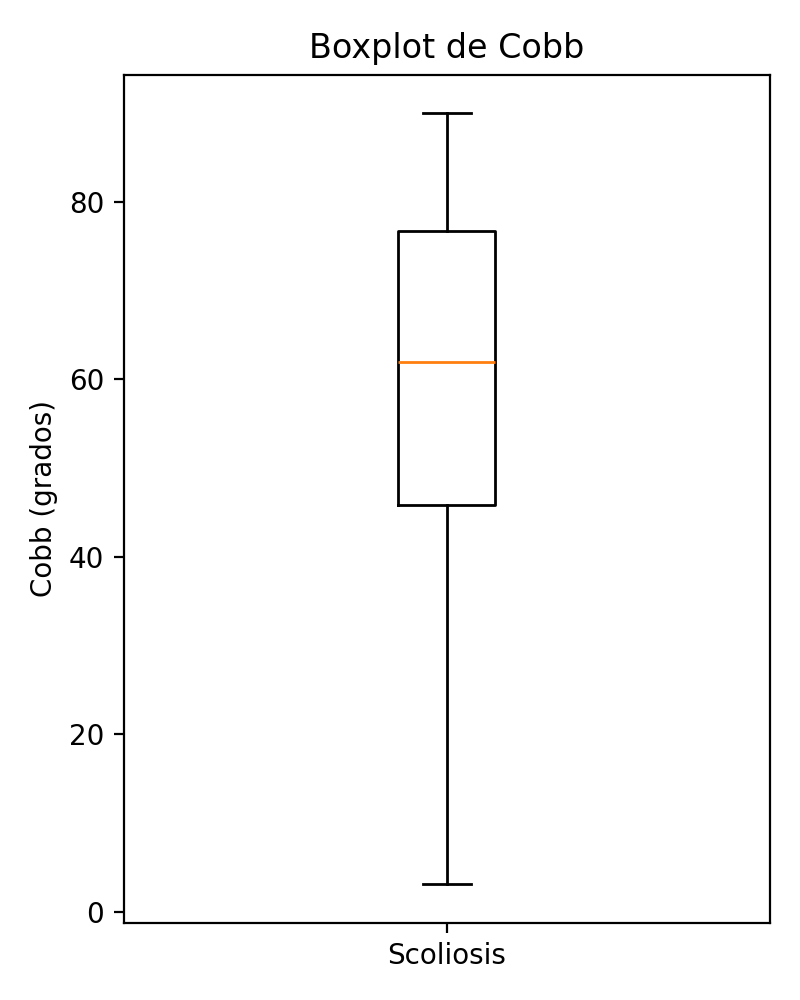
\includegraphics[width=0.48\linewidth]{analysis/figures/cobb_boxplot.png}
    \end{center}
    \textit{Figura.} Distribución del ángulo de Cobb en el subconjunto de escoliosis (histograma y boxplot), útil para interpretar sesgo de severidad y estrategia de validación.

    \item \textbf{Cronograma.}

    Plan tentativo (16 semanas):
    \begin{itemize}[leftmargin=0.6cm]
        \item \textbf{Semanas 1--3:} preparación del dataset, control de calidad y preprocesamiento.
        \item \textbf{Semanas 4--6:} implementación y ajuste del baseline CNN.
        \item \textbf{Semanas 7--9:} integración de descriptores topológicos (TDA).
        \item \textbf{Semanas 10--12:} implementación de Transformer multi-kernel y pruebas iniciales.
        \item \textbf{Semanas 13--14:} experimentos comparativos y ablaciones.
        \item \textbf{Semanas 15--16:} análisis final de resultados, conclusiones y redacción del informe.
    \end{itemize}

    \textbf{Resultados esperados y recursos.} Se espera obtener una mejora medible en segmentación y coherencia anatómica frente a líneas base, junto con una estimación automática más estable del ángulo de Cobb. Para ello se usarán recursos de cómputo en nube con soporte GPU, ejecución distribuida por \textit{workers}, mensajería de eventos (Pub/Sub o SNS/SQS) y seguimiento de experimentos con MLflow.

    \item \textbf{Bibliografía.}

    Referencias preliminares:
    \begin{itemize}[leftmargin=0.6cm]
        \item Ronneberger, O., Fischer, P., \& Brox, T. (2015). \textit{U-Net: Convolutional Networks for Biomedical Image Segmentation}. MICCAI.
        \item Isensee, F., et al. (2021). \textit{nnU-Net: a self-configuring method for deep learning-based biomedical image segmentation}. Nature Methods.
        \item Tao, R., Liu, W., \& Zheng, G. (2022). \textit{Spine-transformers: Vertebra labeling and segmentation in arbitrary field-of-view spine CTs via 3D transformers}. Medical Image Analysis.
        \item Zhang, Y., et al. (2023). \textit{A Spine Segmentation Method under an Arbitrary Field of View Based on 3D Swin Transformer}. International Journal of Intelligent Systems.
        \item Li, X., et al. (2024). \textit{VerFormer: Vertebrae-Aware Transformer for Automatic Spine Segmentation from CT Images}. Diagnostics.
        \item Aydogdu, S., et al. (2024). \textit{Improving Vertebrae Segmentation Using a Centroid Detection-Guided Transformer-Based Network}. IEEE ISBI.
        \item Clough, J. R., et al. (2020). \textit{A Topological Loss Function for Deep-Learning Based Image Segmentation Using Persistent Homology}. IEEE TPAMI.
        \item Hu, X., et al. (2019). \textit{Topology-Preserving Deep Image Segmentation}. NeurIPS.
    \end{itemize}

\end{enumerate}

\end{document}